\newpage
\part{Final Design/Implementation}

    \graphicspath{{images/finalDesign/}}

    \section{Front-End}

        The item on the navigation bar corresponding to the current page goes bold to give the user an indication of the page they are currently viewing.

        \subsubsection{Main Page}

        The final layout of the main page is shown in Fig.~\ref{fig:main_page_layout}. The charts were created with chart.js. When the sliders are moved, the chart is redrawn and the values displayed beside the sliders change accordingly.

        \textbf{outline chart parsing and redraw process}

        \begin{figure}[h]
            \centering
            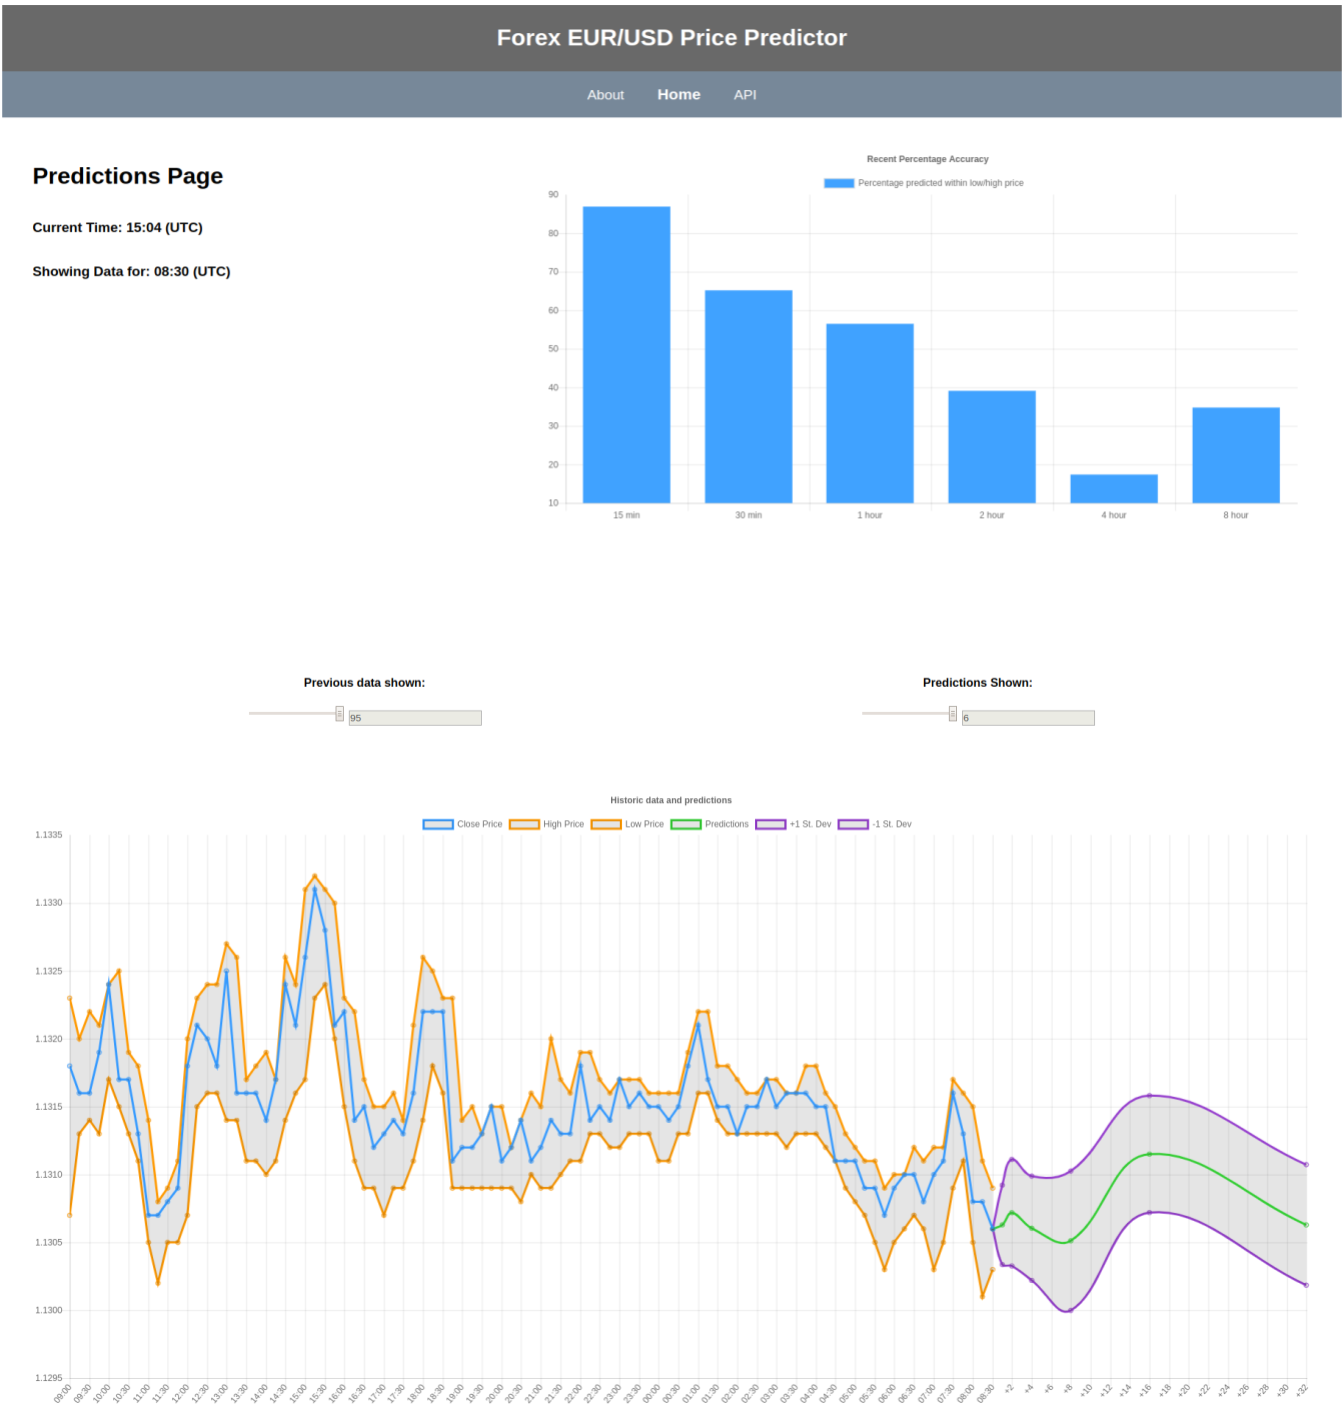
\includegraphics[width=0.8\textwidth]{main page layout.png}
            \caption{Layout of main page}
            \label{fig:main_page_layout}
        \end{figure}

        \subsection{API}

            The final layout of the API page is shown in Fig.~\ref{fig:api_page_layout}

            \begin{figure}[h]
                \centering
                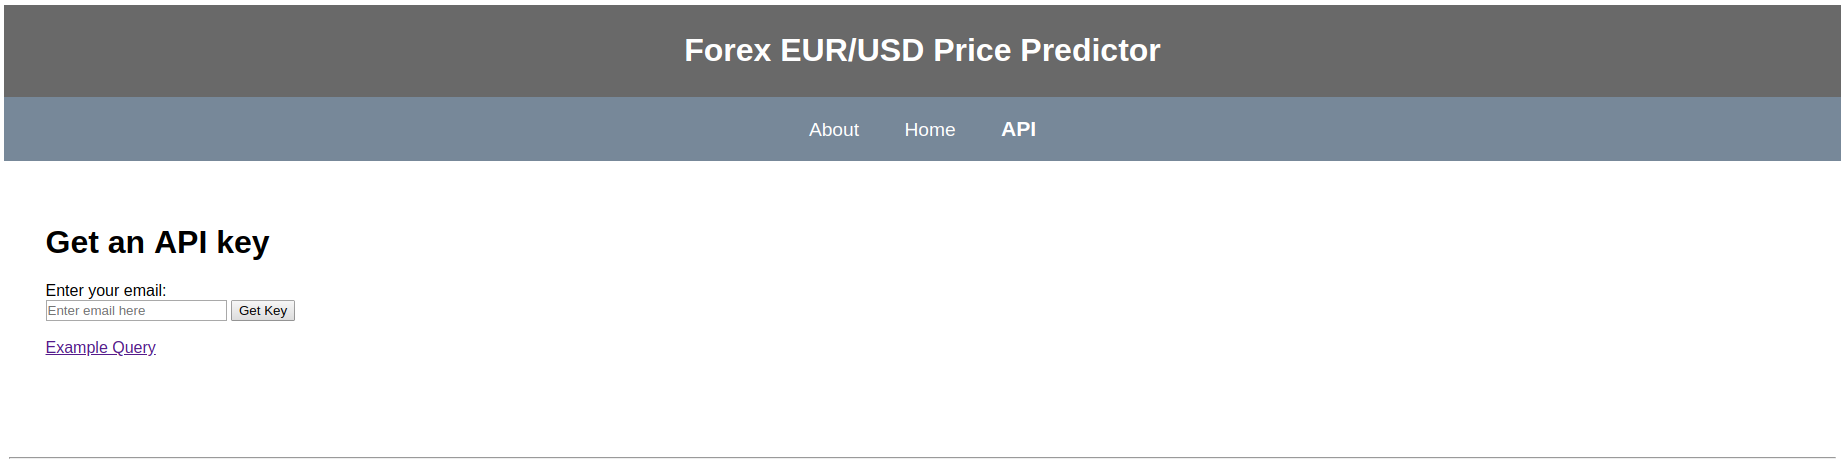
\includegraphics[width=0.8\textwidth]{api page layout.png}
                \caption{Layout of api page}
                \label{fig:api_page_layout}
            \end{figure}

            If a user enters an email whose hash is not found in the database, they will be redirected to the "show key" page, shown in Fig.~\ref{fig:api_show_key}

            \begin{figure}[h]
                \centering
                
\includegraphics[width=0.8\textwidth]{api show key.png}
                \caption{Show key page}
                \label{fig:api_show_key}
            \end{figure}

            If the email hash is found in the database, the page will reload and a message will be displayed above the text field. Fig.~\ref{fig:api_used_email}

            \begin{figure}[h]
                \centering
                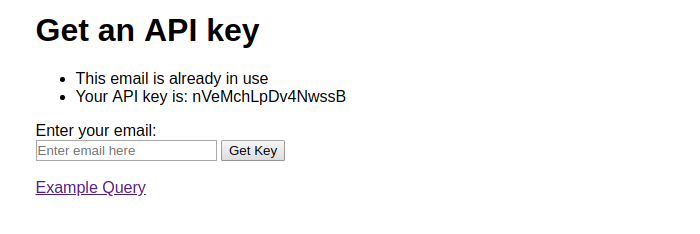
\includegraphics[width=0.8\textwidth]{api used email.png}
                \caption{Used email message}
                \label{fig:api_used_email}
            \end{figure}

            If an invalid email is entered, a javascript alert will be shown and the page reloaded. Fig.~\ref{fig:api_js_alert}
            
            \begin{figure}[h]
                \centering
                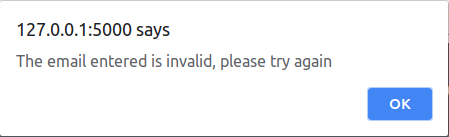
\includegraphics[width=0.8\textwidth]{api js alert.png}
                \caption{Javascript alert}
                \label{fig:api_js_alert}
            \end{figure}
            

            \subsubsection{Hashing}
            As discussed previously hashing should be done client-side to keep user's emails secure. It was decided that md5 would be a good hashing algorithm to use as it is (relatively) secure and quick, so hashing the emails this way would not add a noticeable amount of time to the time it takes for a request to be processed.

            The algorithm for verifying and hashing an email is outlined below:

            \begin{itemize}
                \item \textit{on the submission of a form}
                \begin{itemize}
                    \item \textit{get value entered to the form}
                    \item \textit{if a match is found when the value is tested against an email regex pattern}
                    \begin{itemize}
                        \item \textit{apply the salt to the email and send a post request to the server}
                    \end{itemize}
                    \item \textit{else}
                    \begin{itemize}
                        \item \textit{show a javascript alert to the user, asking them to enter a valid email}
                    \end{itemize}
                \end{itemize}
            \end{itemize}

        \subsection{About Page}

        The final layout of the About page is shown in Fig.~\ref{fig:about_page}. The page includes links to the dataset used to train/test the networks, chart.js and alphavantage.

            \begin{figure}[h]
                \centering
                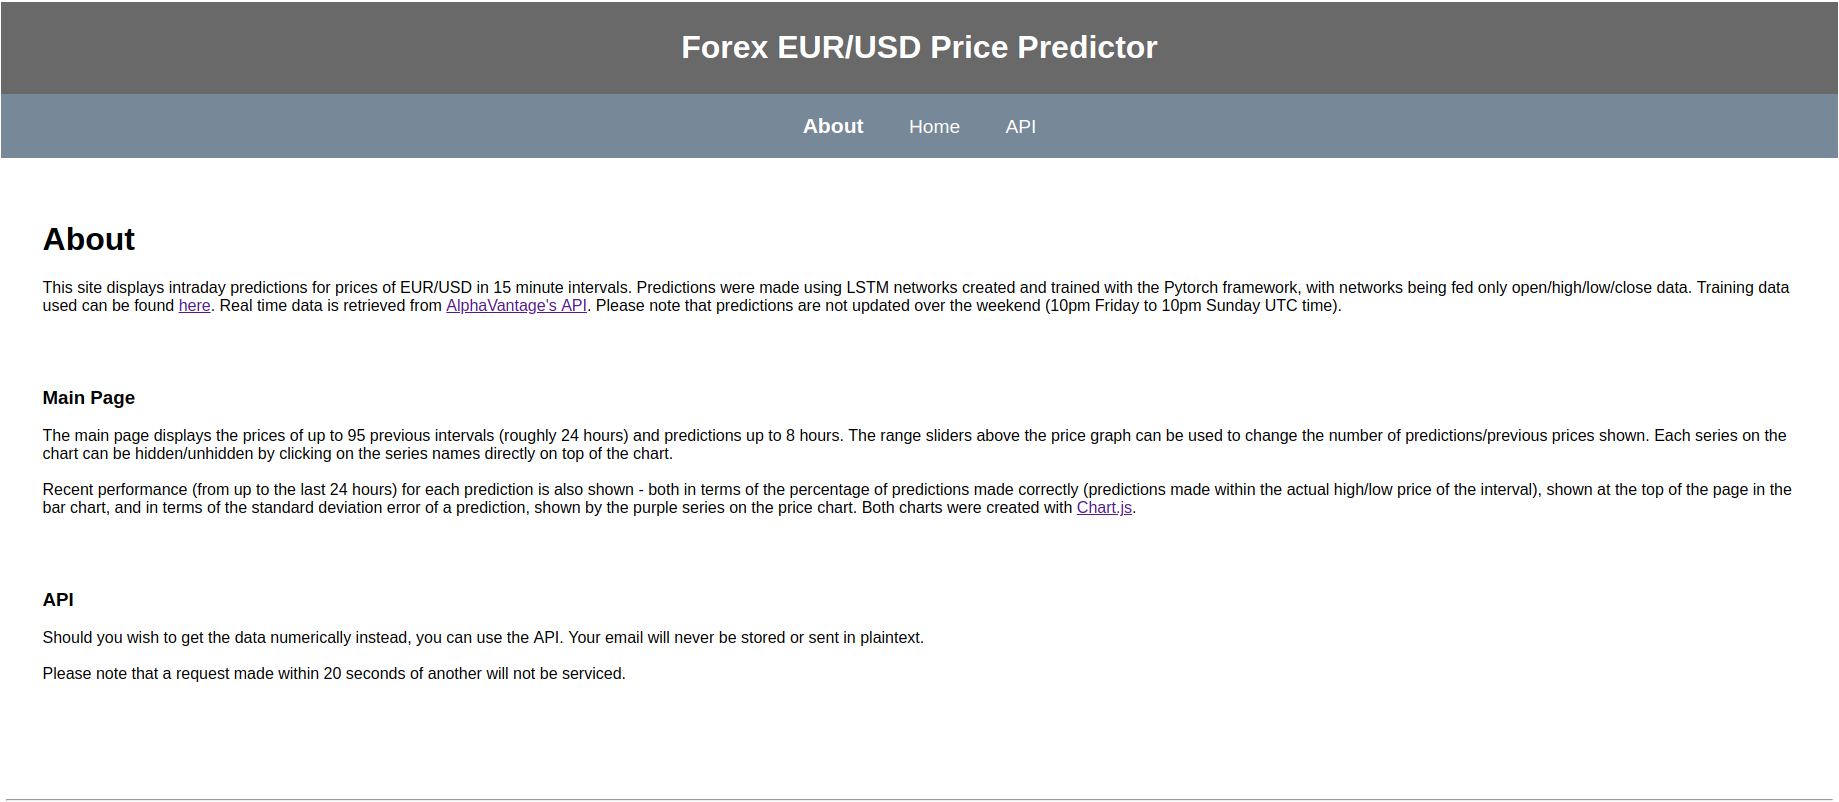
\includegraphics[width=0.8\textwidth]{about page.png}
                \caption{Layout of about page}
                \label{fig:about_page}
            \end{figure}

    \section{Back-End}

        The Site's source code file tree is shown below. \textbf{add site file tree}

        \begin{minted}[tabsize=4, breaklines]{text}
site
|___static 
|   |___json                //all json files used
|   |   |___data.json           //AlphaVantage data file
|   |   |___error.json          //file returned by API if error
|   |   |___invalidGet.json     //file returned by API if bad request
|   |   |___predictions.json    //file of predictions/accuracies
|   |   |___sample.json         //example of data in format of predictions.json
|   |___nets                //trained networks
|       |___  ...
|___templates           //html files returned by app routes
|   |___about.html          //about page
|   |___api.html            //api page
|   |___home.html           //home page
|   |___layout.html         //base html structure that the other pages extend
|   |___showKey.html        //page showing user their API key
|
|___config.py           //site configurations 
|___database.py         //init the database
|___models.py           //SQLAlchemy database table models
|___app.py              //main 
|___api.py              //all logic and routes for the API page and serving API requests
|___update.py           //price and prediction updates
        \end{minted}

        \subsection{Networks}
        
        When training the LSTM, network there still seemed to be a few issues with the validity of predictions - the networks still appeared to be converging on solutions that would more or less quote the most recent close price, and would end up performing worse than the baseline both in terms of percentage accuracy and MSE. 

        While the network didn't appear to be overfitting on training data, it was thought that early stopping could be useful to help make better predictions. By not allowing the network to fully converge on a solution, it was thought that it may be better at predicting trends instead and potentially perform better overall.

        The final networks used had structures and performances as follows. For each timestep, the baseline stats are shown directly above the trained network. All final networks used only one layer of LSTM cells.

        \begin{tabular}{|p{2cm}|p{1.5cm}|p{1.5cm}|p{2.5cm}|p{2.5cm}|}
            \hline
            Timestep & Window Size & Layer number & Percentage Performance & Mean Squared Error\\
            \hline
            \multirow{15 (15*1)}
            & - & - & 91.166 & 0.0047292\\
            & 5 & 20 & 92.586 & 0.0047001\\
            \hline
            \multirow{30 (15*2)}
            & - & - & 91.166 & 0.0091900\\
            & 10 & 20 & 91.979 & 0.0091604\\
            \hline
            \multirow{60 (15*4)}
            & - & - & 91.165 & 0.018476 \\
            & 20 & 30 & 87.311 & 0.018470 \\
            \hline
            \multirow{120 (15*8)}
            & - & - & 91.164 & 0.0047292 \\
            & & & & \\
            \hline
            \multirow{240 (15*16)}
            & - & - & 91.163 & 0.0047292 \\
            & 65 & 30 & 81.197 & 0.076780 \\
            \hline
            \multirow{480 (15*32)}
            & - & - & 0 & 0 \\
            & & & & \\
            \hline
        \end{tabular}

        The network predicting the 8 hour price was the only one not to pass the baseline. It was thought that at least part of this was due to the hardware limitations of the machine being using to train the data. When attempting to train the networks with larger windows i.e. those predicting prices further in the future, the batch size has to be decreased significantly to the point where network predicting the 8 hour price was trained with a batch size \footnote{During training, it is not practical to feed all the test data a network during each iteration (before trying to optimise to the network parameters). Because of this, a percentage of the data is chosen randomly to be fed, giving an approximation of the networks ability. This means the "step" taken by the optimiser will likely not be the most appropriate however overall this saves time during training.} of 3\% instead of a suggested \textbf{find suggested reasonable batch size and citation}.

        As the network performed comparably to the baseline, it was still used in the final solution.

        Given the above, using a machine that has a graphics card with more memory, it is likely that "useful" predictions (predictions that have a lower MSE than the baseline) could have been made. However, there were limitations due to the amount of data AlphaVantage returned (100 timesteps reliably)and so a different real time price source/saving of historic prices would be needed.

        When processing the historic data to feed to the network, a lot of care had to be put in to do this properly. For a given number of timesteps n, there are (n-timeStepToPredict-windowSize) pairs of test data/targets as there is "padding" either side of every "current" price (the last price being fed to the network)

        The algorithm used to get all the data needed for testing/training was as follows: 
        
        \begin{itemize}
            \item retrieve data as list of records from csv
            \item convert the first (length of the returned records - the timeStepToPredict) records to pytorch tensors, take as "inputs"
            \item take the close price of the last (timeStepToPredict + windowsize) records as a pytorch tensor, take as "targets"
            \item get the mean for each window that can be made from the inputs
            \item split means, inputs and targets into training/testing data
        \end{itemize}

        When training, to get each batch, the following algorithm is used:

        \begin{itemize}
            \item 
        \end{itemize}

        \subsection{Updating data}

            The final updating process is shown in Fig.~\ref{fig:update_flowchart}. The main path of the flowchart is shown in bold
            
            \begin{figure}[h]
                \centering
                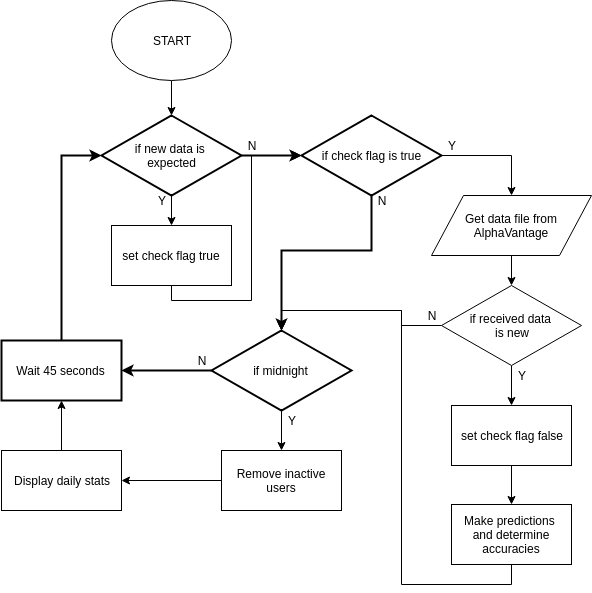
\includegraphics[width=0.9\textwidth]{update flowchart.png}
                \caption{Flowchart of updating process}
                \label{fig:update_flowchart}
            \end{figure}
            
            An example of some of the json data retrieved from AlphaVantage is shown below. 

            \begin{minted}[frame=single, framesep=3mm, linenos=true, xleftmargin=2pt,tabsize=4]{js}
{
    "Meta Data": {
        "1. Information": "FX Intraday (15min) Time Series",
        "2. From Symbol": "EUR",
        "3. To Symbol": "USD",
        "4. Last Refreshed": "2019-03-28 01:15:00",
        "5. Interval": "15min",
        "6. Output Size": "Compact",
        "7. Time Zone": "UTC"
    },
    "Time Series FX (15min)": {
        "2019-03-28 01:15:00": {
            "1. open": "1.1252",
            "2. high": "1.1253",
            "3. low": "1.1246",
            "4. close": "1.1251"
        },
        "2019-03-28 01:00:00": {
            "1. open": "1.1248",
            "2. high": "1.1252",
            "3. low": "1.1245",
            "4. close": "1.1252"
        },
        "2019-03-28 00:45:00": {
            "1. open": "1.1250",
            "2. high": "1.1252",
            "3. low": "1.1246",
            "4. close": "1.1247"
        },
        ...
    }
}
            \end{minted}

            \subsubsection{Getting new Predictions}
        
            To make the design more flexible and easier to update, a general pytorch LSTM network class was defined that could take in all networks of the proposed structure. Each network was saved to a file whose name corresponded to the structure of the network it stored. The name was in the format "priceToPredict-windowSize-LSTMCellNo-LSTMLayerNo.pth" - e.g. "15-10-20-1.pth" is a network that gives predictions for 15 minutes in the future, taking in data from 10 previous timesteps and feeding them to 1 layer of 20 LSTM units. 

            Using the above, the algorithm for getting new predictions is as follows:

            \begin{itemize}
                \item \textit{for each network file path}
                    \begin{itemize}
                        \item \textit{split network file path by '-'}
                        \item \textit{create instance of network with correct structure using the split values}
                        \item \textit{parse trained parameters at the file path to the network }
                        \item \textit{get data according to the window size specified in the file path and normalise the values}
                        \item \textit{feed the data to the network}
                        \item \textit{"un-normalise" the output of the network to get a prediction for the price.}
                    \end{itemize}
            \end{itemize}
            
        
            From a list of all the file paths of networks to be used, every 15 minutes, each file name was used to get the structure of the network, an instance of the LSTM network was initialised using this structure and the trained parameters of the network were loaded into the class instance. Incoming data was then normalised and fed to the network. Once all predictions were made, predictions are saved to the database and the performance of recent predictions were assessed. Finally the json file of predictions and accuracies with the new values.


            \subsubsection{Determining accuracy}
            
            The amount of historic data available at any one time is quite small (previous 100 timesteps) so potentially will not be many recent predictions that can be assessed at any one time e.g. when the site is first run after a period of time offline or on Monday morning where there will not not be any predictions from the past 24 hours to assess. Because of this, an "unbiased estimate" for standard deviation is calculated instead of the raw standard deviation.

            \begin{equation}
            \sigma \approx \sqrt{\frac{n}{n-1}(\frac{\sum x^{2}}{n} - (\frac{\sum x}{n})^{2})}
            \end{equation}

            The formula used is shown above, where x is the absolute error of each prediction and n is the number of predictions in the sample.

            The algorithm for assessing predictions is as follows: 
            \begin{itemize}
                \item \textit{for each prediction timestep - i.e. for each of the 15min, 30min, 1h etc predictions}
                    \begin{itemize}
                        \item \textit{initialise variables totalCorrect, totalError, totalSquaredError}
                        \item \textit{determine the time of prediction furthest back in the past for which there is actual price data}
                        \item \textit{determine the most recent time of prediction for which there is actual price data}
                        \item \textit{query the prediction table for predictions made between the two times calculated above}
                        \item \textit{for each prediction record returned}
                        \begin{itemize}
                            \item \textit{get the relevant prediction}
                            \item \textit{determine the time the prediction was made for}
                            \item \textit{get the actual OHLC prices for that time}
                            \item \textit{if the prediction was within the high/low price}
                            \begin{itemize}
                                \item \textit{add 1 to totalCorrect}
                            \end{itemize} 
                            \item \textit{get the absolute error of the prediction-the actual close price}
                            \item \textit{add this to totalError, add the square of this to totalSquaredError}
                            \item \textit{calculate percentage and unbiased estimate of standard deviation}
                        \end{itemize}
                    \end{itemize}
            \end{itemize}

        \subsection{Database}

        The SQLAlchemy package was used to manage the database. SQLAlchemy allows for the same control that raw SQL offers but has the advantage of allowing interaction with entities as python objects. This helped make requests easier to implement as well as helping to keep code visually consistent.

        Some examples of database queries used throughout the solution are shown below.

        At midnight, daily stats are retrieved and printed to the console. The following requests get these stats, making use of SQL's COUNT, BETWEEN and DISTINCT functions.

        \begin{minted}[frame=single, framesep=3mm, linenos=true, xleftmargin=2pt, tabsize=4, breaklines]{python}
#number users who have signed up in the last day
newSignups = user.query.filter(db.between(user.dateJoined, dayBefore, current)).count()

#total number of users remaining in the database
remainingUsers = user.query.count()

#number of users who have made a request in the last day
activeUsers = apiRequest.query.distinct(apiRequest.user_id) .filter(db.between(apiRequest.dateTime, dayBefore, current)).count()

#total number of requests made in the past day
totalRequests = apiRequest.query.filter(db.between(apiRequest.dateTime, dayBefore, current)).count()

#number of requests that were rejected in the last day 
rejectedRequests = apiRequest.query.filter(apiRequest.served==0) .filter(db.between(apiRequest.dateTime, dayBefore, current)).count()
        \end{minted}
        
        When an API request is made, a "crosstab" query is made to get a user and the time of their last request.

        \begin{minted}[frame=single, framesep=3mm, linenos=true, xleftmargin=2pt, tabsize=4, breaklines]{python}
#get the last most recent user/apiRequest datetime where the user's apikey is equal to the one entered
User = db.session.query(user, apiRequest.dateTime).outerjoin(apiRequest, user.id == apiRequest.user_id).filter(user.apiKey == apiKey).order_by(apiRequest.dateTime.desc()).first()
        \end{minted}

        \subsection{API}

        Luckily, flask makes sending static files to a user very simple so implementing the sending of the json data was very straightforward - the majority of the work came in the user validation and ensuring requests weren't being made too frequently.

        When a post request is sent back to the server, the server checks the form returned with the following algorithm.

        \begin{itemize}
            \item \textit{if the isValid property of the form is 1}
            \begin{itemize}
                \item \textit{query the user table for the first entry with emailHash = emailHash returned}
                \item \textit{if the query returns an entry}
                \begin{itemize}
                    \item \textit{refresh the page with a message telling the user the email is already being used and give them their api key}
                \end{itemize}
                \item \textit{else if nothing is returned}
                \begin{itemize}
                    \item \textit{generate a random alphanumeric api key.}
                    \item \textit{redirect user to a page displaying the api key and some information about usage.}
                \end{itemize}
            \end{itemize}
        \end{itemize}

        When an API request is sent to the server (a request is made to the api/data route), the following algorithm is used to determine what data is returned to the user.

        \begin{itemize}
            \item \textit{if the request is made with an "apikey" argument}
            \begin{itemize}
                \item \textit{if the apikey = "testkey"}
                \begin{itemize}
                    \item \textit{return sample.json}
                \end{itemize}
                \item \textit{else}
                \begin{itemize}
                    \item \textit{make a crosstab query to get a user with the apikey entered and the time of their last request}
                    \item \textit{if the query returns an entry i.e. apikey was found in the database}
                    \begin{itemize}
                        \item \textit{if this is the first request made by the user i.e. no datetime was returned in the query OR the last request made was more than 20 seconds ago, return predictions.json}
                        \item \textit{add entry to the apiRequest table}
                    \end{itemize}
                \end{itemize}
            \end{itemize}
            \item \textit{else i.e. if the query returned None OR the user has already made a request in the last 20 seconds OR no API key was given as an argument}
            
            \begin{itemize}
            \item \textit{return invalidGet.json}
            \end{itemize}            
        \end{itemize}

        An example of the returned predictions file is shown below

        \inputminted[frame=single, framesep=3mm, linenos=true, xleftmargin=2pt, tabsize=4, breaklines]{js}{../source/site/static/json/sample.json}

        If the user has not entered an API key, if the entered key was invalid or if a request was made in the last 20 seconds, the following file is sent 
        
        \inputminted[frame=single, framesep=3mm, linenos=true, xleftmargin=2pt, tabsize=4, breaklines]{js}{../source/site/static/json/invalidGet.json}

        If there is an error in writing to / querying the database, the following file is sent.
        \inputminted[frame=single, framesep=3mm, linenos=true, xleftmargin=2pt, tabsize=4, breaklines]{js}{../source/site/static/json/error.json}
